\chapter{Sanskrit documents}

In \textsc{Pāli\,Platform\,4}, Sanskrit learning tools have been added. The main purpose of the addition is not to make a kind of \textsc{Sanskrit\,Platform} to facilitate Sanskrit studies like we have seen in the main functions of \textsc{Pāli\,Platform} for Pāli studies, but rather to help Pāli learners grasp the essence of Sanskrit language as fast as possible. As your study goes deeper, involving with Sanskrit seems inevitable. Having similar learning tools for Sanskrit is really beneficial to serious Pāli learners. However, as the things turn out, Sanskrit functions in the program are also helpful to Sanskrit students, particularly as a tool for quick looking up.

Apart from Sanskrit dictionaries we have already seen in Chapter \ref{chap:dict}, the first tool in this part is the Sanskrit document viewer. The only source of Sanskrit documents we use is the GRETIL's bulk collection of Sanskrit data.\footnote{\url{gretil.sub.uni-goettingen.de/gretil/1\_sanskr.zip}} This file contains all Sanskrit documents available in GRETIL. Before using the collection, we have to download it first by the program's downloader invoked by menu Sanskrit > {\faSix \symbol{"F381}} Download Sanskrit documents. The downloader has functions like that of the DPD (see further in Chapter \ref{chap:dpd}).\footnote{Manual installation of the documents is also easy. Just place \texttt{1\_sanskr.zip} in directory \texttt{data/text/skt}.} Once you have the data file of Sanskrit documents, you can read \emph{most} of them.

\boxnote{Not all texts in the Sanskrit collection are read by the program. Only those under directory \texttt{transformation} are. These texts are made unified in structure, so easier to access and manipulate.}

To open the document index, use menu Sanskrit > {\ppicons H}\ GRETIL Sanskrit documents. Then a window like Figure \ref{fig:sanskrit-docindex} will show up.

\begin{figure}[!hbt]
\centering
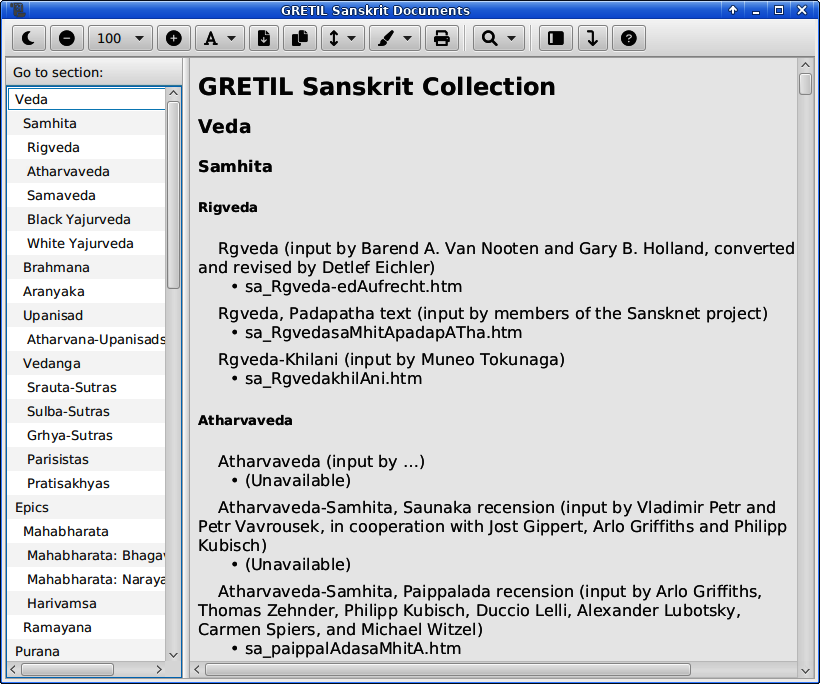
\includegraphics[width=0.9\linewidth]{images/sanskrit-docindex.png}\\
\caption{Index of GRETIL Sanskrit documents}
\label{fig:sanskrit-docindex}
\end{figure}

The navigator of the index can be opened by {\ppicons A}\ button. The information of each entry is taken verbatim from the GRETIL's index. If a document is available to read, you will see its filename (encoded in SLP1 and ending with \texttt{.htm}), otherwise it is marked with \emph{Unavailable}.\footnote{The unavailable entries are either documents not under directory \texttt{transformation} and those external documents outside GRETIL. In the former case, you can really see the text by exploring the collection zip file yourselves. To see the missing information, please look at the GRETIL's index directly.} To open a document, just click its filename (see Figure \ref{fig:sanskrit-docopen}).

\begin{figure}[!hbt]
\centering
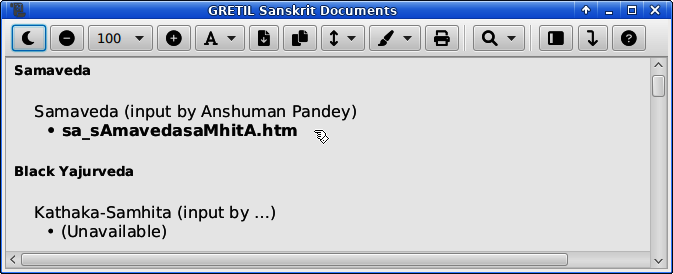
\includegraphics[width=0.9\linewidth]{images/sanskrit-docopen.png}\\
\caption{Opening a Sanskrit document}
\label{fig:sanskrit-docopen}
\end{figure}

\dothis{To open a Sanskrit document, click its filename (starting with \texttt{sa\_} and ending with \texttt{.htm}), otherwise it is unavailable.}

Once a document is opened, you will feel familiar because the viewer has similar functionality as you have seen in Pāli text viewers. Because of differences in structure, there are a few key functions that you can do with this simple viewer.

Each text in this collection basically has two parts: \emph{header} and \emph{text}. The header contains information about the text (metadata). You can jump to the former part by {\faSix \symbol{"F015}} button, and the latter by {\faSix \symbol{"F70E}} button.

Dictionary lookup works as you expect when a word is selected. If the exact entry is not found, the nearest is shown, marked by an asterisk (*). Figure \ref{fig:sanskrit-doclookup} shows a word lookup in Sāmavedasaṃhitā.\footnote{This text is very handy to test because it is short and has position near the top of the index.}

\begin{figure}[!hbt]
\centering
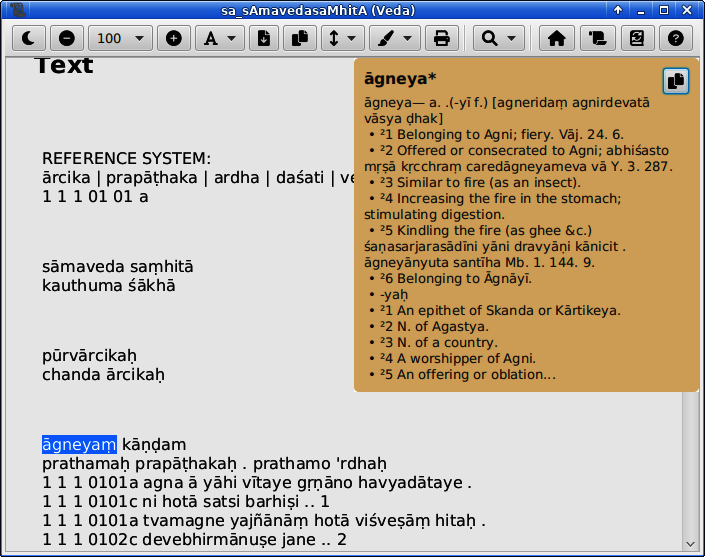
\includegraphics[width=0.9\linewidth]{images/sanskrit-doclookup.png}\\
\caption{Dictionary lookup in a Sanskrit document}
\label{fig:sanskrit-doclookup}
\end{figure}

The dictionary used in the lookup can be set in Settings as shown in Figure \ref{fig:settings-sktdict}. When a new dictionary is selected while a viewer is being opened, you may need to update the dictionary by hitting {\ppicons I}\ button.

\begin{figure}[!hbt]
\centering
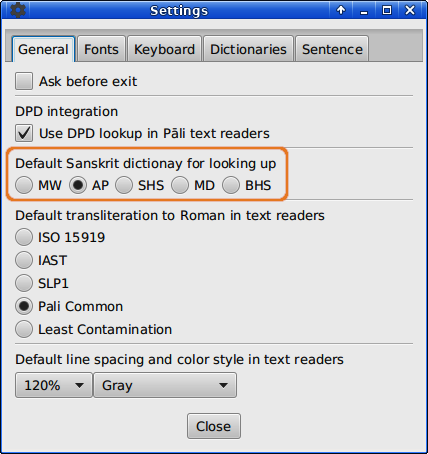
\includegraphics[width=0.6\linewidth]{images/settings-sktdict.png}\\
\caption{Default Sanskrit dictionary for word lookup}
\label{fig:settings-sktdict}
\end{figure}

Other basic functions of text viewer can be used as well, such as string finding tool (\texttt{Ctrl-F}) shown in Figure \ref{fig:sanskrit-docfind}.

\begin{figure}[!hbt]
\centering
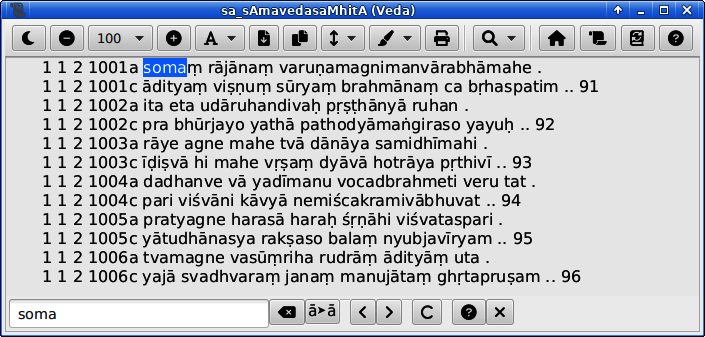
\includegraphics[width=0.9\linewidth]{images/sanskrit-docfind.png}\\
\caption{String finding in a Sanskrit document}
\label{fig:sanskrit-docfind}
\end{figure}

Moreover, like texts in Pāli collections, you can treat this Sanskrit collection as a corpus (abbreviated as \emph{SKT}). That is to say, you can find a document by Document Finder (Chapter \ref{chap:finder}), index and search for a string with Lucene Finder (Chapter \ref{chap:lucene}), and list all tokens with Term Lister (Chapter \ref{chap:lister}). However, because texts in this Sanskrit collection have various formatting styles, and are contaminated with other languages sometimes, they cannot be transliterated by the viewer.\footnote{A portion of text can be copied and converted nonetheless in Text Editor.}

